\section{Coordinate Systems}

In circular accelerators, particle dynamics are represented using a traveling coordinate system.
A reference orbit is determined by the lattice and its magnet strengths, forming the
\textit{optics}. In the case of a synchrotron, like the LHC, where the particles return to their
original location after some turns, the reference orbit is also called the closed orbit.  





% ============================================
%               Frenet-Serret
% ============================================
\subsection{\review{Frenet-Serret System}}

The Frenet-Serret coordinate system moves along the ring on the reference orbit. The coordinates are
then transverse: $x$ and $y$, and longitudinal in the direction of travel: $s$.
Figure~\ref{fig:coordinate_systems:frenet_serret} shows those coordinates.

\begin{figure}[H]
    \centering
    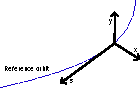
\includegraphics[width=0.5\textwidth]{images/frenet.pdf}
    \caption{Frenet-Serret coordinate system, commonly used in accelerator physics. The system moves
    along the reference orbit.}
    \label{fig:coordinate_systems:frenet_serret}
\end{figure}

This coordinate system is widely used to simply describe a either an element's or a particle's
position in the accelerator. Without any explicit mention, those are coordinates used in this
thesis. It is frequent to use the variable $z$ to refer to either $x$ or $y$ in equations.



% ============================================
%               Linear Lattice 
% ============================================
\subsection{Linear Lattice}


% ========================
% Courant-Snyder Parameters
\subsubsection{\review{Courant-Snyder Parameters}}
\label{section:courant_snyder}

A circular accelerator is composed of many multipoles of different orders. A basic
design only requires dipoles and quadrupoles in order to operate. Dipoles are used to bend the
particles in order to form the ring, whereas quadrupoles are used to focus the beam to a focal
point, similar to light optics.
Those elements can be arranged in a particular order, to form a FoDo cell. Such cells present an
alternating placement of focusing an defocusing quadrupoles with dipoles in between, as shown in
Fig.\ref{fig:coordinate_systems:fodo}, and are usually repeated many times along the ring.

\begin{figure}[htb]
    \centering
    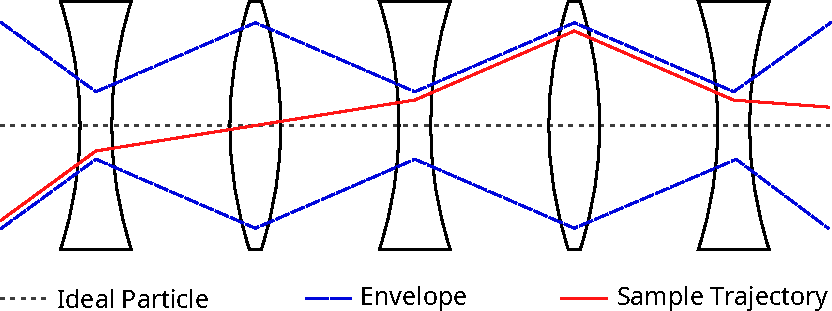
\includegraphics[width=0.8\textwidth]{images/fodo_drawing.pdf}
    \caption{Line composed of FoDo cells, a basic cell present in most accelerators, composed of a
    Focusing and a Defocusing quadrupole. The envelope is a factor of the $\beta$-function and the
    action $J$.}
    \label{fig:coordinate_systems:fodo}
\end{figure}

A lattice composed of only dipoles and quadrupoles, is referred to as a \textit{linear} lattice.
In a synchrotron, a circular particle accelerator, particles undergo transverse and longitudinal 
oscillations. As such, particles do not go back to their initial position before a certain number
of turns. Taking into account those oscillations, the phase-space ellipse of a particle at a 
position $s$ in the ring can be described with a new system: the Courant-Snyder parameters, also
know as Twiss parameters or the \textit{optics functions}~\cite{courant_theory_1958}, as shown in
Fig.~\ref{fig:coordinate_systems:twiss}.\\

\begin{figure}[htb]
    \centering
    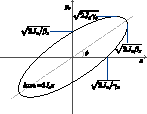
\includegraphics[width=0.6\textwidth]{images/phase_space.pdf}
    \caption{Phase-space ellipse of a linear machine, parametrized by the Courant-Snyder
    parameters $\alpha$, $\beta$ and $\gamma$.}
    \label{fig:coordinate_systems:twiss}
\end{figure}

$J$, the action, an invariant of motion at a given energy, is related to the other quantities by:

\begin{equation}
    J_z = \frac{1}{2} (\gamma_z \cdot z^2 + 2 \alpha_z p_z \cdot z + \beta_z p_z^2).
    \label{eq:coordinate_systems:action}
\end{equation}

The action can be related to the area in phase space, called the emittance: $\epsilon = 2J$.
As the $\beta$ parameter varies along the ring, it is referred to as the $\beta$-function and is
related to the amplitude of the oscillations. Thus, the smaller is the $\beta$-function, the
smaller is also the envelope of the beam.
The number of oscillations per turn is called the \textit{tune}, and is closely related to the
$\beta$-function:

\begin{equation}
    Q_{x,y} = \frac{1}{2 \pi} \oint \frac{1}{\beta_{x,y}(s)} \diff s.
    \label{eq:coordinate_systems:tune}
\end{equation}


It is common to express the position of a particle using \textit{action-angle} variables, allowing
to switch between the Courant-Snyder parameters and the Frenet-Serret system:

\begin{equation}
    \begin{aligned}
    z   &= \sqrt{2J_z \beta_z} \cos{\phi_z} \\
    p_z &= - \sqrt{\frac{2J_z}{\beta_z}} \left( sin{\phi_z} + \alpha_z \cos{\phi_z}\right).
    \end{aligned}
    \label{eq:coordinate_systems:action_angle}
\end{equation}


% ========================
% Linear Transfer Map
\subsubsection{Linear Transfer Map}




% ============================================
%             Non-Linear Lattice 
% ============================================
\subsection{Non-Linear Lattice}

% ========================
% Lie Algebra
\subsubsection{Lie Algenra}

So far, Courant-Snyder parameters were a good way to describe the distribution of positions and
velocities of particles in the transverse plane. One caveat of using this formalism is that it is 
restrained to linear optics and does not describe non-linear beam dynamics such as resonances or 
the effects arising from an arrangement of several multipoles together.

One way to describe such effects is to introduce Lie Algebra~\cite{dragt_overview_2013}, a vector
space $\mathfrak{g}$ equipped with a binary operation called the \textit{Lie bracket} and denoted
$[x, y]$ for two vectors $x$ and $y$. Any vector space ~equipped with a Lie bracket (or
multiplication rule) satisfying the following conditions is called a Lie algebra:

\begin{itemize}
    \item Bilinearity:
    \begin{equation}
        \begin{aligned}
        \relax[ax+by, z] &= a[x,z] + b[y,z], \\
        [z, ax+by] &= a[z,x] + b[z,y], \quad \forall x,y,z \in \mathfrak{g}~\text{and}~a,b~\text{scalars}
        \label{eq:coordinates:bilinearity}
        \end{aligned}
    \end{equation}

    \item Alternativity:
    \begin{equation}
        [x,x] = 0, \quad \forall x \in \mathfrak{g}
    \end{equation}

    \item Anticommutativity:
    \begin{equation}
        [x,y] = -[y,x], \quad \forall x,y \in \mathfrak{g}
    \end{equation}

    \item The Jacobi identity:
    \begin{equation}
        [x,[y,z]] + [y, [z,x]] + [z, [x,y]] = 0, \quad \forall x,y,z \in \mathfrak{g}
        \label{eq:coordinates:jacobi_identity}
    \end{equation}
\end{itemize}




% ========================
% Poisson Brackets
\subsubsection{Poisson Brackets}

To create a Lie algebra, an operation satisfying those conditions needs to be found. In accelerator
physics, \textit{Poisson brackets} are chosen~\cite{dragt_overview_2013,roy_analysis_1992}. Let's
consider position and momentum coordinates $q_i \cdots q_n$ and $p_i \cdots p_n$  of a
2n-dimensional phase space. Usually, those would be $x, y, p_x \text{ and } p_y$ for transverse
coordinates. The Poisson brackets of two functions $f$ and $g$ if then defined by:

\begin{equation}
    [f,g] = \sum^n_{i=1} \frac{\partial f}{\partial q_i} \frac{\partial g}{\partial p_i}
                       - \frac{\partial f}{\partial p_i} \frac{\partial g}{\partial q_i}.
\end{equation}



% ========================
% Lie Operator
\subsubsection{Lie Operator}

Given a function $f$, a differential operator called \textit{Lie operator} is defined, and is closely
related to the previously seen Poisson bracket:

\begin{equation}
    :f: = \sum^n_{i=1} \frac{\partial f}{\partial q_i} \frac{\partial}{\partial p_i}
                     - \frac{\partial f}{\partial p_i} \frac{\partial}{\partial q_i}.
\end{equation}

The action of this operator on a function $g$ is equivalent to the Poisson brackets, as in:

\begin{equation}
    :f:g = [f,g].
\end{equation}

A particular power series of this Lie operator can now be defined, called \textit{Lie
transformation}:

\begin{equation}
    \begin{aligned}
        e^{:f:}g &= \sum_{l=0}^\infty \frac{1}{l!} :f:^l g \\
                 &= g + [f,g] + \frac{1}{2!}[f, [f, g]] + \cdots .
    \end{aligned}
\end{equation}



% ========================
% Non-Linear Transfer Map
\subsubsection{Non-Linear Transfer Maps}

As introduced \todo{before}, the dynamics of a particle beam in a circular accelerator can be
described by \textit{transfer maps}. A symplectic \textit{One Turn Map} $\mathcal{M}$ that also
includes $N$ non-linear elements is defined~\cite{dragt_overview_2013} as:

\begin{equation}
    \mathcal{M} = e^{:h_N:} \cdot e^{:h_{N-1}:} \cdots e^{:h_1:} \cdot \mathcal{R}
\end{equation}

where $\mathcal{R}$ is a matrix describing the linear motion over one turn and the $h_i$ terms
representing the Hamiltonian of each non-linear elements of the machine.
Via the Baker-Campbell-Hausdorff (BCH)\todo{citation} theorem, previous Lie transformations can be combined and
simplified:

\begin{equation}
    e^{:h_1:} \cdot e^{:h_2:} = e^{:h:}
\end{equation}
with 
\begin{equation}
    \begin{aligned}
        h =& h_1 + h_2 \\
           & + \frac{1}{2} [h_1, h_2] \\
           & + \frac{1}{12} [h_1, [h_1, h_2]] - \frac{1}{12} [h_2, [h_1, h_2]] + \cdots.
    \end{aligned}
    \label{eq:coordinates:bch}
\end{equation}

The one turn map is thus expressed as a single Lie transformation:

\begin{equation}
    \mathcal{M} = e^{:h:} \cdot \mathcal{R}.
\end{equation}

In most cases, were the non-linear perturbations are small, the above series converges quickly
and only the two first terms of Eq.~\eqref{eq:coordinates:bch} are
used~\cite{carlier_nonlinear_2020-1}. The resulting expression is then more elegant, being a simple
sum of the Hamiltonians of the $N$ non-linear elements:

\begin{equation}
   \mathcal{M} = e^{:h_1 + h_2 + \cdots + h_N:} \cdot \mathcal{R}.
\end{equation}

It is though to be noted that in this thesis experimental measurements show the evidence of higher
order contributions. In order to fully understand the combined effect of multipoles, the BCH
expansion needs to be expended further than the first two terms.


% ========================
% Normal Form
\subsubsection{Normal Form}

